\documentclass{beamer}
\usepackage{fontspec}
\usepackage{xunicode}
\usepackage{xltxtra}
\usepackage{hyperref}
\hypersetup{colorlinks=true}
%\usepackage[latin1]{inputenc}

\usepackage{graphicx}
\usepackage{float}

\newcommand\song{\fontspec[ExternalLocation=/usr/local/share/fonts/msfonts/]{simsun.ttc}}
\newfontfamily\monaco{Monaco}
\setromanfont{Monaco}

\title[Tools: SSH, latex and others]{Tools: ssh, latex and others}
\author{yangpeng@knet.cn}
%% \institute{\song 技术部}
\date{Dec 13, 2011}


\usetheme{Warsaw}


\begin{document}



\begin{frame}
  \titlepage
\end{frame}



\begin{frame}
  \frametitle{Menu}
  \begin{itemize}

  \item SSH forwarding and \emph{fanqiang} \\
  \item latex \\
  \item other \\

  \end{itemize}
\end{frame}




\begin{frame}
  \frametitle{SSH forwarding}

  \begin{itemize}
  \item local forwarding \\
  \item remote forwarding \\
  \item \emph{dynamic forwarding} \\
  \end{itemize}


  resource on the site: 
  \href{https://www.ibm.com/developerworks/cn/linux/l-cn-sshforward/}{ibm developerworks} \\



\end{frame}





\begin{frame}
  \frametitle{local forwarding}

  ssh -L port:host:hostport xxxx@xxxxxxx \\

  \pause
  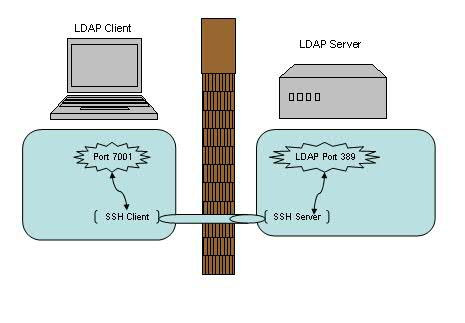
\includegraphics[width=0.8\textwidth,height=0.6\textheight]{local.jpg}

  \pause
  on pc-after-NAT: python -m SimpleHTTPServer \\
  \pause
  on yangpeng@knet: ssh -NL 8000:localhost:8000 root@111.12.148.115 \\

\end{frame}


\begin{frame}
  \frametitle{remote forwarding}

  ssh -R port:host:hostport xxxx@xxxxxxx \\

  \pause
  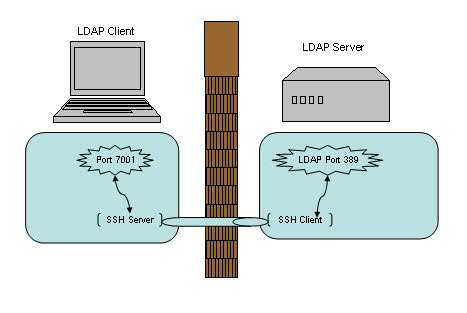
\includegraphics[width=0.8\textwidth,height=0.6\textheight]{remote.jpg}

  \pause
  on yangpeng@knet: ssh -NR 4000:localhost:22 root@218.241.108.183 \\
  \pause
  on 183: ssh -p 4000 yangpeng@localhost \\

\end{frame}



\begin{frame}
  \frametitle{dynamic forwarding}

  \emph{fxxking the gfw} \\

  \begin{itemize}
  \item linux, mac os x \\
  \item ipad, android \\
    \pause
  \item windows \\
  \end{itemize}

\end{frame}






\begin{frame}
  \frametitle{latex: Donald Knuth}

  \emph{this very pdf is made by latex} \\



\end{frame}






\begin{frame}
  \frametitle{chrome extension}

  \begin{itemize}
  \item \href{http://code.google.com/p/switchysharp/wiki/SwitchySharp_GFW_List_2}{Proxy SwitchySharp} \\
    \pause
  \item \href{http://vimium.github.com/}{Vimium} \\
    \pause
  \item \href{https://chrome.google.com/webstore/detail/kjhmfidomefgpbbebodnbakelpabilga/details}{A Little Privacy} \\
    \pause
  \item \href{https://lastpass.com/}{LastPass} \\
    \pause
  \item \href{http://readitlaterlist.com/}{Orbvious Interest(readitlater)} \\
    \pause
  \item \href{https://chrome.google.com/webstore/detail/mgijmajocgfcbeboacabfgobmjgjcoja}{Google Dictionary (by Google)} \\
  \end{itemize}

\end{frame}




\begin{frame}
  \frametitle{more other}

  \begin{itemize}
  \item google code as disk:
  \href{http://code.google.com/p/confile/source/browse/\#svn\%2Ftrunk}{confile}
  \item \href{https://www.google.com/reader/view/\#overview-page}{google reader}
  \item \href{http://www.ted.com/}{ted}
\item \href{http://stackoverflow.com/}{stackoverflow}
  \end{itemize}

\end{frame}

















\begin{frame}
  \frametitle{thanks}

  ideas for life \\

\end{frame}






%% \begin{frame}{Persistence}
%%   http://redis.io/topics/persistence \\
%%   \pause
%%   \begin{block}{Snapshotting}
%%     \begin{itemize}
%%     \item conf: save 60 1000 \\
%%     \item command: SAVE, BGSAVE \\
%%     \end{itemize}
%%   \end{block}

%%   \pause
%%   \begin{block}{Append-only file:  fully-durable}
%%     \begin{itemize}
%%     \item conf: \\
%%       appendonly yes \\
%%       appendfsync always \\
%%       appendfsync everysec \\
%%       appendfsync no \\
%%     \item Log rewriting \\
%%       command: BGREWRITEAOF \\
%%     \end{itemize}
%%   \end{block}

%% \end{frame}







\end{document}

